\section{Anexo}
\subsection{Presupuesto} 
\noindent A continuación, se muestra el presupuesto a partir de las horas invertidas descritas en la planificación, dando un total de \$ $3.842.227$ pesos. 
\begin{table}[H]
\centering
\caption{Presupuesto del proyecto}
\label{tab: presupuesto}
\resizebox{\columnwidth}{!}{%
\begin{tabular}{clc|c|c|c|}
\hline
\multicolumn{1}{|l|}{} & \multicolumn{1}{l|}{\textbf{Actividades}} & \textbf{Horas} & \textbf{UF/hr} & \textbf{UF*} & \textbf{CLP} \\ \hline
\multicolumn{1}{|c|}{\multirow{8}{*}{\textbf{Costo ingeniería}}} & \multicolumn{1}{l|}{Planificación} & $7$ & $0.6$ & $4.2$ & $151.687$ \\
\multicolumn{1}{|c|}{} & \multicolumn{1}{l|}{Mediciones} & $9$ & $1$ & $9$ & $325.044 $\\
\multicolumn{1}{|c|}{} & \multicolumn{1}{l|}{Modelación} & 1$8 $& $0.8$ & $14.4$ & $520.070$ \\
\multicolumn{1}{|c|}{} & \multicolumn{1}{l|}{Análisis de datos} & $6$ & $1$ & $6$ & $216.696$ \\
\multicolumn{1}{|c|}{} & \multicolumn{1}{l|}{Diseño de propuesta} & $24$ & $1$ & $24$ & $866.784$ \\
\multicolumn{1}{|c|}{} & \multicolumn{1}{l|}{Análisis de propuesta} & $12$ & $0.8$ & $9.6$ & $346.713$ \\
\multicolumn{1}{|c|}{} & \multicolumn{1}{l|}{Cotización de propuesta} & $8$ & $0.6$ & $4.8$ & $173.356$ \\
\multicolumn{1}{|c|}{} & \multicolumn{1}{l|}{Redacción de informe} & $26$ & $0.6$ & $15.6$ & $563.409$ \\ \hline
\multicolumn{1}{|c|}{\multirow{2}{*}{\textbf{Costo operacional}}} & \multicolumn{1}{l|}{Arriendo de equipos} &  &  & $1.7$ & $60.000$ \\
\multicolumn{1}{|c|}{} & \multicolumn{1}{l|}{Traslados} &  &  & $0.1$ & $5.000$ \\ \hline
\multicolumn{1}{l|}{} & \multicolumn{1}{l|}{\textbf{Total}} & $110$ &  & $89.3$ & $3.228.762$ \\ \cline{2-6} 
\multicolumn{1}{l}{} &  &  & IVA ($19$\%) & $17$ & $613.465$ \\ \cline{4-6} 
\multicolumn{1}{l}{} &  &  & Total (con IVA) & $106.3$ & $3.842.227$ \\ \cline{4-6} 
\end{tabular}%
}
\end{table}

*\textit{Considerando el valor en UF correspondiente a la fecha del $28$ de agosto de $2023$ es de \$ $36.116$ CLP.}


\subsection{Marco teórico}
\subsubsection{Ruido de fondo (RdF)}
El ruido de fondo es el sonido presente en una sala cuando no hay actividad o no está presente la fuente a evaluar. Este ruido puede ser causado por sistemas de climatización, instalaciones eléctricas o hidráulicas, e incluso ruido externo como el tráfico.

\begin{itemize}

    \item \textbf{Curvas NC}: son curvas de referencia que representan los límites de ruido aceptables en un espacio según su uso. Un recinto se considera que cumple una especificación NC determinada (por ejemplo, NC-$15$, NC-$20$, etc.) cuando los niveles de ruido de fondo, medidos en diferentes bandas de frecuencia, están por debajo de la curva NC correspondiente para todas las frecuencias entre $63$ Hz y $8$ kHz (ver figura \ref{fig:curvas NC}).\cite{carrion1990diseno}
    \begin{figure}[H]
        \centering
        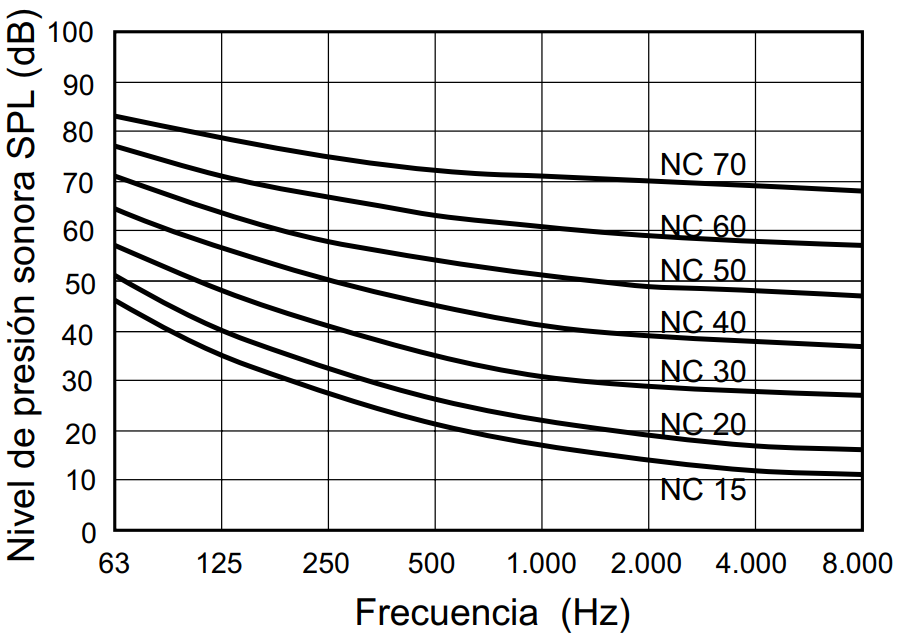
\includegraphics[width=8cm]{Imagenes/MarcoTeorico/CurvaNC.png}
        \caption{Curvas NC (``Noise Criteria'')}
        \label{fig:curvas NC}
    \end{figure}
    En la tabla \ref{tab:recomendaciones Curva NC} se muestran las curvas NC recomendadas para diferentes tipos de recinto, junto con su equivalencia en dBA.
    \begin{table}[H]
        \centering
        \caption{Curvas NC recomendadas y niveles de ruido de fondo equivalentes en dBA }
        \label{tab:recomendaciones Curva NC}
        \begin{tabular}{|l|c|}
        \hline
        \textbf{Tipos de recinto} & \textbf{\begin{tabular}[c]{@{}l@{}}Curva NC\\ recomendada\end{tabular}} \\ \hline
        Fábricas para ingeniería pesada & $55$ - $75$ \\ \hline
        Fábricas para ingeniería ligera & $45$ - $65$ \\ \hline
        Cocinas industriales & $40$ - $50$ \\ \hline
        Recintos deportivos y piscinas & $35$ - $50$ \\ \hline
        Grandes almacenes y tiendas & $35$ - $45$\\ \hline
        Restaurantes, bares, cafeterías y cafeterías privadas & $35$ - $50$  \\ \hline
        Oficinas mecanizadas & $40$ - $50$  \\ \hline
        Oficinas generales & $35$ - $45$  \\ \hline
        Despachos, bibliotecas, salas de justicia y aulas & $30$ - $35$ \\ \hline
        viviendas, dormitorios & $25$ - $35$ \\ \hline
        Salas de hospitales y quirófanos & $25$ - $35$  \\ \hline
        Cines & $30$ - $35$\\ \hline
        Teatros, salas de juntas, iglesias & $25$ - $30$ \\ \hline
        Salas de conciertos y teatros de ópera & $20$ - $25$ \\ \hline
        Estudios de registro y reproducción sonora & $15$ - $20$ \\ \hline
        \end{tabular}
    \end{table}

    \item \textbf{Curvas NR}: Las curvas NR son estándares que muestran los niveles de ruido de fondo aceptables en recintos. Se dividen en números NR (como NR-15, NR-25, NR-35), que indican el nivel máximo de ruido permitido en decibelios (dB) según el propósito del espacio.
En la figura \ref{NR}, se muestran las curvas NR de evaluación de ruido y en la tabla \ref{tabla} , figuran los valores recomendados del índice de NR para diferentes locales.\cite{Recuero}

\begin{figure}[H]
    \centering 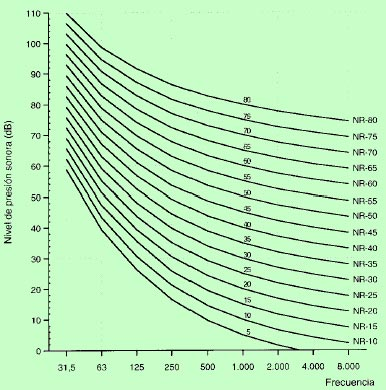
\includegraphics[scale=0.6]{Imagenes/MarcoTeorico/NR.jpg}
    \caption{Curvas NR}
    \label{NR}
\end{figure}

\begin{table}[H]
\centering
\caption{Valores recomendados de índice NR para distintos locales.}
\label{Valores recomendados de NR}
\resizebox{15 cm}{!}{%
\begin{tabular}{|l|c|}
\hline
\multicolumn{1}{|c|}{\textbf{Tipos de recintos}}                                                       & \textbf{Rangos de niveles NR} \\ \hline
Talleres                                                                                               & $60$ - $70$                       \\ \hline
Oficinas mecanizadas                                                                                   & $50$ - $55$                       \\ \hline
Gimnasios, piscinas, salas de deporte, pasillos                                                                  & $40$ - $50$                       \\ \hline
Restaurantes, bares y cafeterías                                                                       & $35$ - $45$                       \\ \hline
Despachos, bibliotecas, salas de justicias                                                             & $30$ - $40$                       \\ \hline
\begin{tabular}[c]{@{}l@{}}Cines, hospitales, iglesias, pequeñas salas y aulas de conferencias \end{tabular} & $25$ - $35$                       \\ \hline
\begin{tabular}[c]{@{}l@{}}Estudio de televisión, grandes salas de conferencias\end{tabular} & $20$ - $30$                       \\ \hline
Sala de conciertos, teatros                                                                            & $20$ - $25$                       \\ \hline
Clínicas, recintos para audiometrías                                                                   & $10$ - $20$                       \\ \hline
\end{tabular}%
}
\label{tabla}
\end{table}
    
\end{itemize}

\subsubsection{Tiempo de reverberación (TR)}
El tiempo de reverberación $T_{60}$ es el tiempo que tarda el sonido en decaer $60$ dB en un espacio cerrado. Este parámetro es importante en el diseño de un sistema de refuerzo sonoro, ya que afecta la claridad, inteligibilidad y calidad del sonido en un recinto.

\begin{itemize}
    \item $T_{30}$: Es una expresión del $T_{60}$ que mide el tiempo que demora el sonido en decaer $30$ dB. El valor $T_{30}$ se entrega ya multiplicado por el factor correcto para medir la que sería la caída por $60$ dB.
    \item Formula de Sabine: Uno de los modelos para calcular el tiempo de reverberación es la fórmula de Sabine. La cual es calculada según lo indicado en la ecuación \ref{eq:T60}. \cite{sabine1922collected}
    \begin{equation} \label{eq:T60} 
     T_{60}=0.161 \cdot \frac{V_{t}}{S_{t} \bar{\alpha}}
    \end{equation}

    donde:
    \begin{itemize}
        \item $V_t$ es el volumen total de la sala
        \item $S_t$ es la superficie total de la sala
        \item $\bar{\alpha}$ es la absorción media de la sala
\end{itemize}
    \item $RT_{mid}$: Es la media aritmética de los valores de tiempo de reverberación correspondientes a las bandas de $500$ Hz y $1$ kHz. En general, el valor más adecuado de $RT_{mid}$ depende del volumen del recinto y de la actividad a la que este destinado este. En la tabla \ref{tab:rtmid recomendado por tipo de sala} se muestran valores recomendados de $RT_{mid}$, para diferentes tipos de salas en el supuesto que estén ocupadas. \cite{carrion1990diseno}
    \begin{table}[H]
        \centering
        \begin{tabular}{|l|c|}
        \hline
             \textbf{Tipo de sala} &  $RT_{mid}$\textbf{, sala ocupada}\\ \hline
             Sala de conferencia& 
             $0.7$ - $1.0$\\
             Cine             & $1.0$ - $1.2$\\
             Sala polivalente & $1.2$ - $1.5$\\
             Teatro de ópera & $1.2$ - $1.5$\\
             Sala de conciertos (música de cámara) & $1.3$ - $1.7$\\
             Sala de conciertos (música sinfónica) & $1.8$ - $2.0$\\
             Iglesia/catedral (órgano y canto coral) & $2.0$ - $3.0$\\
             Locutorio de radio & $0.2$ - $0.4$\\ \hline
        \end{tabular}
        \caption{Valores de $RT_{mid}$ recomendados en función del tipo de sala (recintos ocupados)}
        \label{tab:rtmid recomendado por tipo de sala}
    \end{table}
    En el caso de salas de salas de conferencia/aulas el $RT_{mid}$ recomendado, considerando volúmenes entre los $100$ y $10000$ $m^3$, es entre los valores de:
    \[0.7 \leq RT_{mid} \leq 1 s \]

    \item Claridad: La claridad se refiere a cómo se distribuye la energía del sonido en un espacio. En términos simples, se mide la relación entre el sonido directo y las primeras reflexiones (llamada energía temprana) en comparación con la energía que llega después. En acústica, se utiliza el parámetro $C_{50}$ para evaluar la claridad en entornos destinados a la voz y el $C_{80}$ para la música. Estos valores se obtienen de manera logarítmica y se calculan para un rango de frecuencias entre $125$ y $4000$ Hz.\cite{carrion1990diseno}
    \begin{equation}
      C_{50}= 10 log_{10} \left[\int_0^{50 ms}[g(t)]^2 dt/\int_{50 ms}^{\infty}[g(t)]^2 dt\right]  
    \end{equation}
    \begin{equation}
      C_{80}= 10 log_{10} \left[\int_0^{80 ms}[g(t)]^2 dt/\int_{80 ms}^{\infty}[g(t)]^2 dt\right]  
    \end{equation}
    Marshall, define valores apropiados de $C_{50}$ para el habla y $C_{80}$ para distintos tipos de música, descritos en la figura \ref{fig:Recomendaciones C50 C80} \cite{marshall1994}
    \begin{figure}[H]
        \centering
        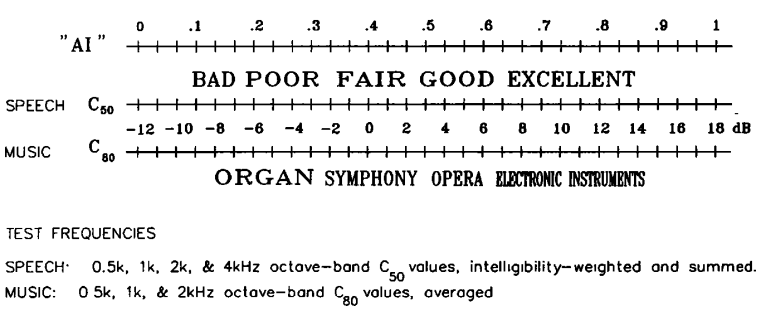
\includegraphics[scale=0.5]{Imagenes/MarcoTeorico/Recomendaciones C50-C80.png}
        \caption{Recomendaciones de claridad para el habla y música}
        \label{fig:Recomendaciones C50 C80}
    \end{figure}
    \item Definición: El parametro llamado definición se determinó para evaluar la cantidad de energía temprana, el cual se deriva directamente de la respuesta impulso $g(t)$ en la siguiente ecuación:
    \begin{equation}
        D_{50}= \left[\int_0^{50 ms}[g(t)]^2 dt/\int_{0}^{\infty}[g(t)]^2 dt\right] 
    \end{equation}
    Ambas integrales deben incluir el sonido directo, cuya llegada al oyente determina el tiempo $t = 0$. Obviamente, D será del $100\%$ si la respuesta al impulso no contiene componentes con retardos superiores a $50$ ms. \cite{Kuttruff_2017} 

    %insertar figura de Relación entre inteligibilidad de sílabas y definición.
    
    \item STI: Es el índice de transmisión del habla el cual indica el entendimiento de la palabra y sus valores oscilan entre los $0$ y $1$, que evalúa la inteligibilidad en el recinto, siendo los valores cercanos a 0 deficientes y los valores cercanos a $1$ una inteligibilidad excelente. Según la normativa ISO $9921$ \cite{ISO9921} los valores clasificarían como se indica en la tabla \ref{tab: rango STI}. 

\begin{table}[H]
    \centering
    \caption{Rango de STI según ISO $9921$}
    \label{tab: rango STI}
    \begin{tabular}{|c|c|}
    \hline
    \textbf{Rango de inteligibilidad} & \textbf{STI} \\ \hline
    Excelente                &     $>0.75$     \\ \hline
    Bueno                    & $0.60$ - $0.75$ \\ \hline
    Razonable                & $0.45$ - $0.60$ \\ \hline
    Pobre                    & $0.30$ - $0.45$ \\ \hline
    Malo                     & $<0.3$ \\ \hline
    \end{tabular}
\end{table}
\end{itemize}


\subsection{Posiciones de mediciones de Tiempo de reverberación}\label{subsec: posiciones RT}
A continuación se pueden observar la distribución de las posiciones de fuente y micrófono para las mediciones de tiempo de reverberación.
\begin{figure}[H]
    \centering
    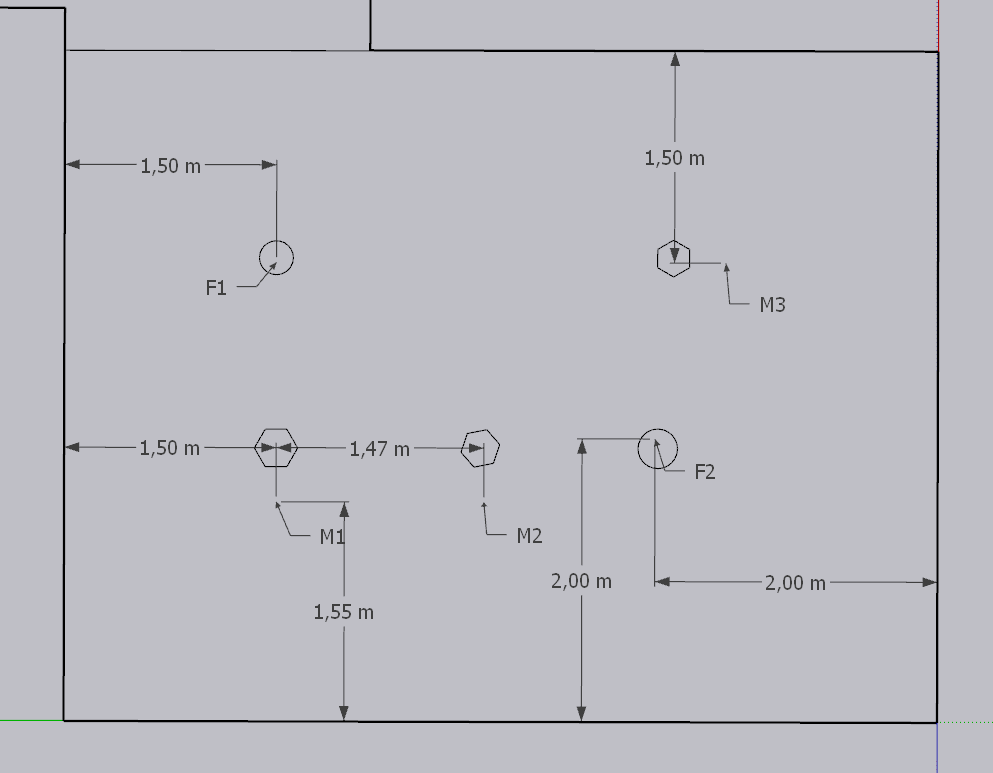
\includegraphics[scale=0.4]{Imagenes/PosicionesRT/Posiciones Sala 1.png}
    \caption{Posiciones de fuente y micrófono para sala de reunión 1}
    \label{fig: posiciones sala1}
\end{figure}

\begin{figure}[H]
    \centering
    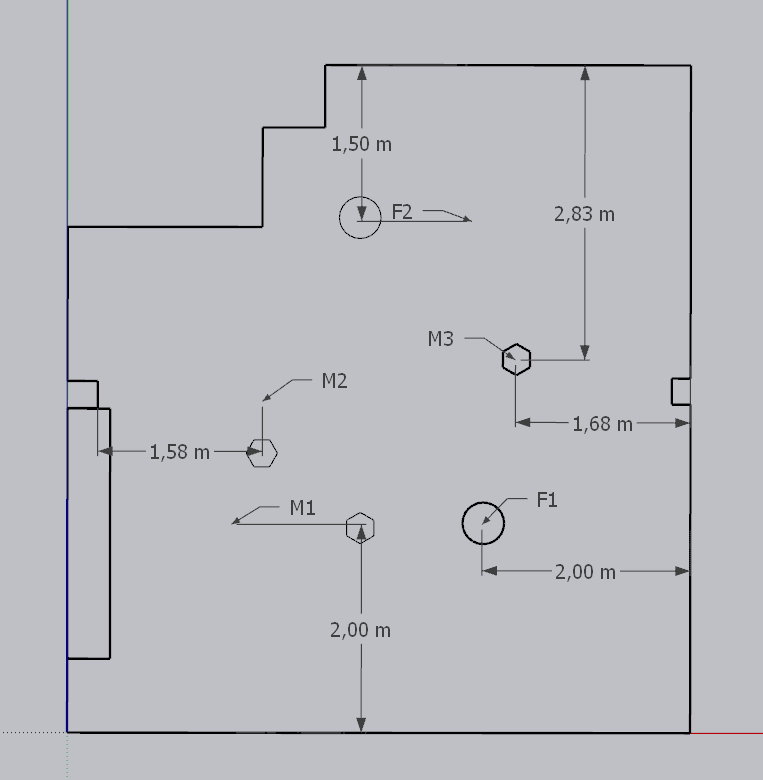
\includegraphics[scale=0.4]{Imagenes/PosicionesRT/Posiciones Sala 2.png}
    \caption{Posiciones de fuente y micrófono para sala de reunión 2}
    \label{fig: posiciones sala2}
\end{figure}

\begin{figure}[H]
    \centering
    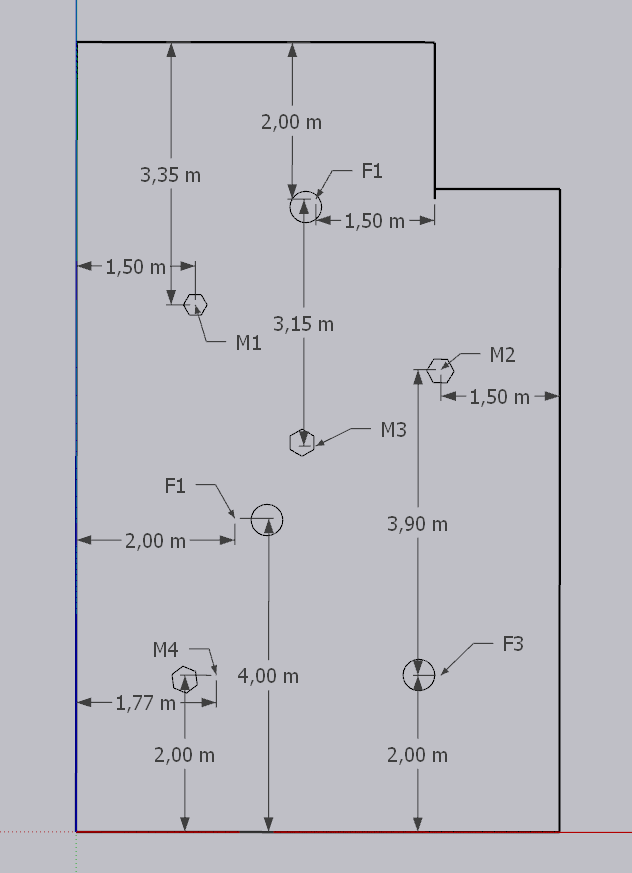
\includegraphics[scale=0.4]{Imagenes/PosicionesRT/Posiciones Sala OCV.png}
    \caption{Posiciones de fuente y micrófono para sala de ensayo}
    \label{fig: posiciones sala OCV}
\end{figure}